\documentclass[10pt,oneside]{article}
\usepackage{amsmath} % Simbolos refinados de matemáticas
\usepackage{graphicx} % Incluir imágenes
\usepackage{subcaption} % Poder usar subfiguras
\usepackage{amsfonts}
\usepackage{amssymb} % Los simbolos el los conjuntos numéricos

% Opciones de lenguaje usando polyglossia (defino dos para este documento)
\usepackage{polyglossia}
\setmainlanguage{spanish}
\setotherlanguage[variant=american]{english}


% El sistema de bibliografá es Biber (no necesitas BibTeX)
\usepackage[
  backend=biber
]{biblatex}
\addbibresource{biblio.bib}

% Márgenes y tamaño del papel
\usepackage[
  letterpaper,
  left=1cm,
  right=1cm,
  top=1.5cm,
  bottom=1.5cm
]{geometry}

% Poner los links en azul y definir los metadatos del pdf
\usepackage[
  final,
  unicode,
  colorlinks=true,
  citecolor=blue,
  linkcolor=blue,
  plainpages=false,
  urlcolor=blue,
  pdfpagelabels=true,
  pdfsubject={Cálculo},
  pdfauthor={José Doroteo Arango Arámbula},
  pdftitle={Tarea 1},
  pdfkeywords={UNAM, FES Acatlán, 2021-I}
]{hyperref}

% Tablas con estilo profesional
\usepackage{booktabs}

% Para poner algortmos en pseudo código
\usepackage{algpseudocode}
\usepackage{algorithm} %Ambiente flotante para los algoritmos
%Hacer los comentarios en el pseudocodigo como en C++
%\algrenewcommand{\algorithmiccomment}[1]{\hskip3em$//$ #1}

% Definición del encabezado y del pies de página
\usepackage{lastpage}
\usepackage{fancyhdr}
\fancyhf{}
\pagestyle{fancy}
\fancyhf{}
\fancyhead[L]{Cálculo I} %Nombre de la materia
\fancyhead[C]{José Doroteo Arango Arámbula} % Nombre del alumno
\fancyhead[R]{\href{mailto:panchovilla@gmail.com}{panchovilla@gmail.com}} % Email
\fancyfoot[R]{Profesor: Dr. Enrique Graue Wiechers}
% https://tex.stackexchange.com/questions/227/how-can-i-add-page-of-on-my-document
\fancyfoot[C]{\thepage\ of \pageref*{LastPage}}
%\fancyfoot[C]{ of }
\fancyfoot[L]{Grupo: 1154} % Grupo
\renewcommand{\headrulewidth}{2pt} 
\renewcommand{\footrulewidth}{2pt}

\usepackage[newfloat=true]{minted} %Para insertar código fuente en algún lenguaje de programación
% Requiere que comiples usando:
% $xelatex -shell-escape input.tex

% Para el correcto funcinamiento, esta plantilla debe compilarse asi:
% 1 XeLaTeX
% 2 Biber 
%    Antes de 20.04 esta herramineta no estaba en los repositorios oficiales de Ubuntu
%    ver: https://tex.stackexchange.com/questions/154751/biblatex-with-biber-configuring-my-editor-to-avoid-undefined-citations/154763#154763)
% 3 XeLaTex
% 4 XeLateX
% 5 ViewPDF

\author{José Doroteo Arango Arámbula} % Again, no utf8 I do not know why
\title{Tarea 1}
% Si por alguna razón la fecha que desaes que aparezca no es la de hoy
% \usepackage{datetime}
% \newdate{date}{06}{09}{2012}
% \date{\displaydate{date}}
\date{\today}

% Configuracion del entorno minted para poner código fuente
\DeclareCaptionFormat{mitedFormat}{%
    \textbf{#1#2}#3}
\DeclareCaptionStyle{minetdStyle}{skip=0cm,width=.85\textwidth,justification=centering,
  font=footnotesize,singlelinecheck=off,format=mitedFormat,labelsep=space}
\newenvironment{mintedCode}{\captionsetup{type=listing,style=minetdStyle}}{}

\usepackage{dirtytalk} %For using qutation marks (usa comillas in spanish)

% Cambia el nombre de la etiqueta. Afecta a todos los codigos minted del codumento
\SetupFloatingEnvironment{listing}{name=Código}
% Opciones de minted para el lenguaje C++
\setminted[cpp]{frame=lines,framesep=0.25cm,baselinestretch=1,fontsize=\scriptsize,breaklines}
% Cuando lo hagas dentro de un parrafo el tamaño de fuente debe ser normal
\setmintedinline[cpp]{fontsize=auto}

\usepackage{csquotes} % Por que si no esta presnte AQUI polyglosia tira un warning

\begin{document}
\maketitle
\thispagestyle{fancy} %Para que los fancy headers esten desde la primera página
% El cuerpo de la tarea esta en este otro archivo
El siguiente texto esta en ingles: \textenglish{Hello world!}
\begin{enumerate}
 \item 
En éste capítulo se presentan varios ejemplos de muchas matemáticas.
Primero, se puede crear una ecuación simple de la siguiente manera:
 \begin{equation}
 \label{eq:elipse}
 \frac{x^{2}}{a^{2}} + \frac{y^{2}}{b^{2}} = 1
 \end{equation}
Y podemos hacer una referencia a ella en el texto de la siguiente manera: La  ecuación \eqref{eq:elipse} representa una elipse.
Si no queremos que las ecuaciones esten numeradas podemos hacer:
 \begin{equation}
 \nonumber
 \binom{n}{k} = \frac{n!}{k!(n-k)!} 
 \end{equation}
 También se pueden insertar ecuaciones dentro de un párrafo, por ejemplo: $\forall x \in \mathbb{R}$.
Se pueden poner links a un sitio web de la siguiente manera:
Para aprender acerca de integrales y sumatorias puedes leer el siguiente \href{https://en.wikibooks.org/wiki/LaTeX/Mathematics#Sums_and_integrals}{wikilibro} o puedes buscarlo en \url{www.google.com}.
Nótese que la segunda forma cambia la fuente del texto.
 
 \item Éste es un ejemplo de una función con casos, como si fuera una \emph{pdf}.
 \begin{equation}
  \label{eq:pdf}
  f(y) =
  \begin{cases}
    \frac{1}{25} y & \quad \text{if } 0 \leq y < 5 \\
    \frac{2}{25} - \frac{1}{25} y & \quad \text{if } 5 \leq y < 10 \\
    0 & \quad \text{if } y < 0 \text{ or } y > 10
  \end{cases}
 \end{equation}
Éste es un ejemplo de paréntesis que ajustan su tamaño automáticamente:
 \begin{equation}
  \nonumber
  P\left(A=2\middle|\frac{A^2}{B}>4\right)
 \end{equation}
Finalmente, pongo un ejemplo de cómo escribir una serie de pasos matemáticos usando el entorno: \verb|align|.
Poner $*$ dentro del entorno te permite omitir los números
\begin{align*}
P\left(X \leq 3 \right) &= \int_{0}^{3} \frac{1}{25} y \,\mathrm{d}y \\
     &= \left. \frac{1}{25} \cdot \frac{1}{2} \, y^{2} \right|_0^3 \\
     &= \frac{1}{25} \left( \frac{1}{2} \, 9 - \frac{1}{2} \, 0 \right) =
     \frac{1}{25} \cdot \frac{9}{2} = \frac{9}{50} \approx 0.18 
\end{align*}

 \item En este ejercicio hay ejemplos de como poner figuras.
La manera más común es que las figuras aparezcan centradas junto con su pie de figura.
 
\begin{figure}[htb]
  \centering
  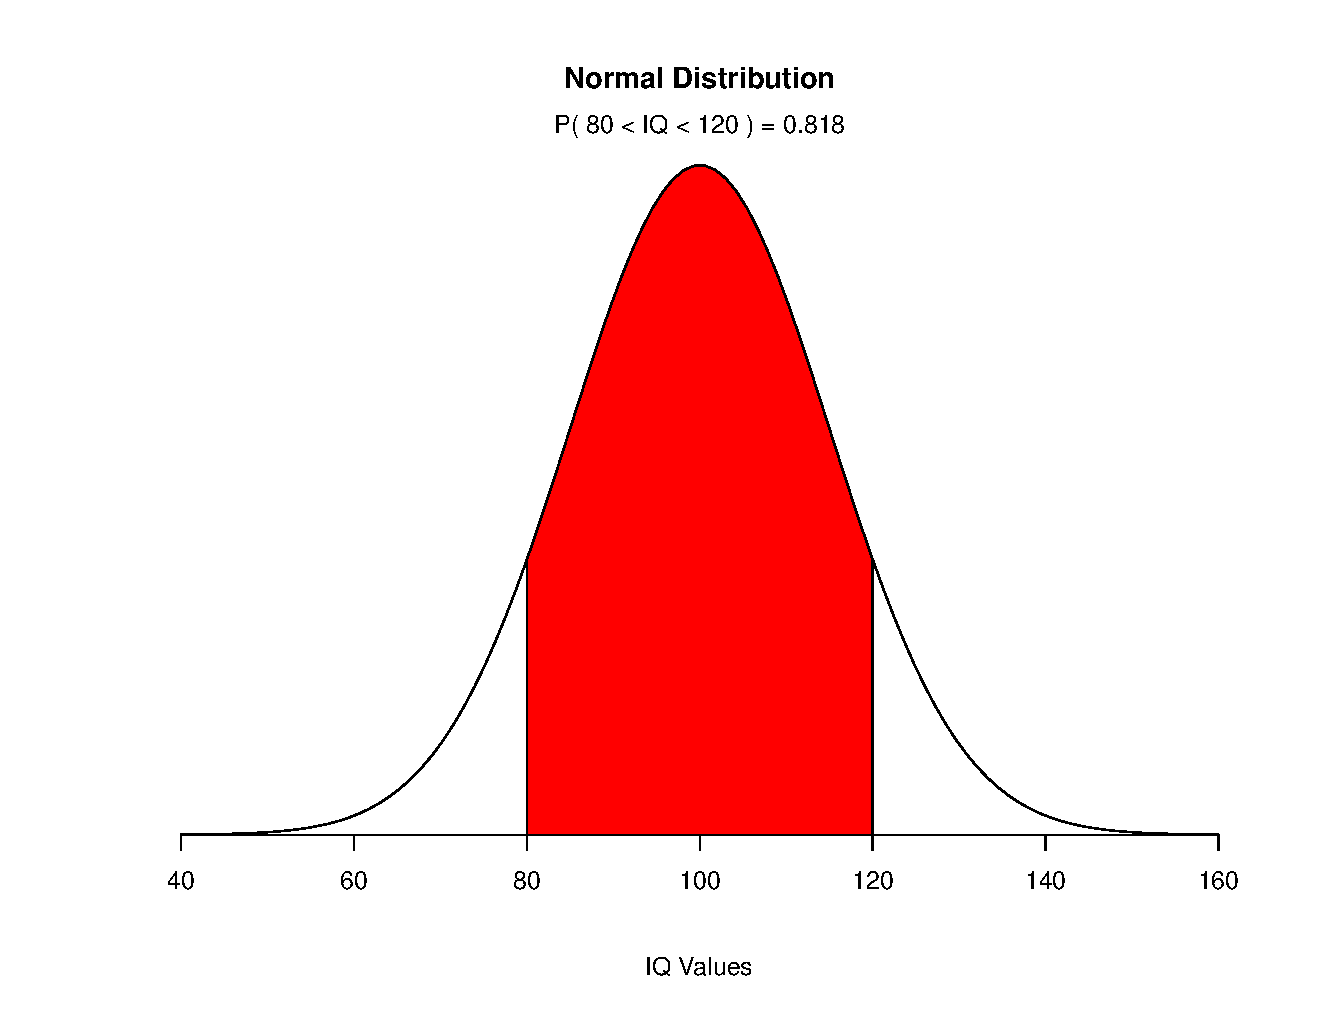
\includegraphics[width=0.45\textwidth]{img/normal}
  \label{fig:one}
\caption[Distribución normal]{Gráfica de una distribución normal. Fue creado usando el siguiente \href{https://www.statmethods.net/advgraphs/probability.html}{script en R}.}
\end{figure}

Por regla general, lo mejor es usar imágenes de tipo vectorial.
Mi tipo de formato preferido es \verb|*.eps| y recomiendo usar \href{https://ipe.otfried.org/}{IPE} o \href{https://inkscape.org/}{InkScape}, pero otros formatos vectoriales populares para imágenes son el \verb|*.pdf| y \verb|*.svg|.

\item También es posible poner figuras, compuestas de varias subfiguras.
Cada subfigura tiene su propio pié y hay un pié de fígura extra para todo el grupo.
Posteriormente, es posible referirse a toda la figura así: Véase la  Figura~\ref{fig:two} ó referirte a una subfigura así:
Vea la Sub Fígura~\ref{fig:2b}.

\begin{figure}[htp]
 \centering
 \begin{subfigure}[b]{0.2\textwidth}
   
\includegraphics[width=\textwidth]{img/ambiente}
   \caption{Reflexión ambiental.}
 \label{fig:2a}
 \end{subfigure}
~
 \begin{subfigure}[b]{0.2\textwidth}
   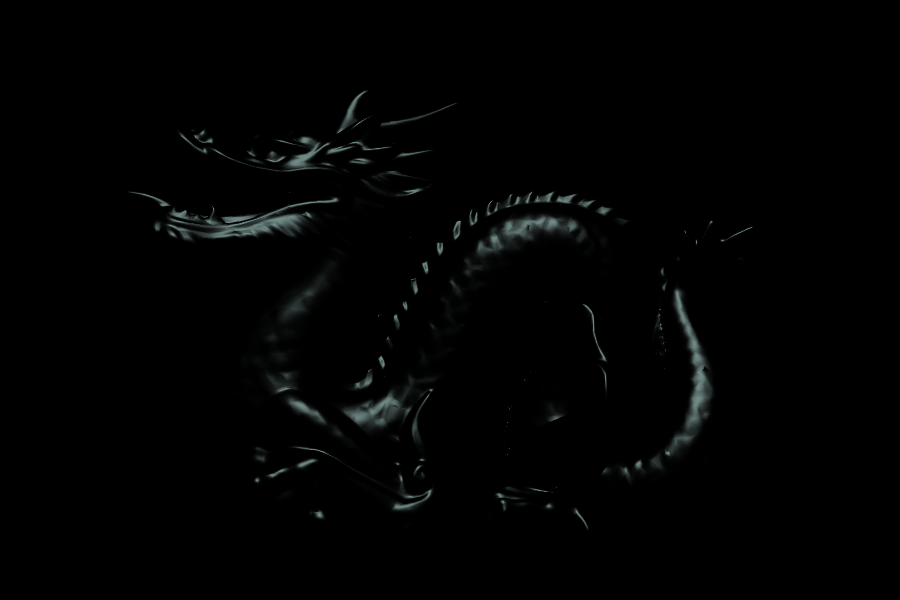
\includegraphics[width=\textwidth]{img/especular}
   \caption{Reflexión especular.}
   \label{fig:2b}
 \end{subfigure}
~
 \begin{subfigure}[b]{0.2\textwidth}
   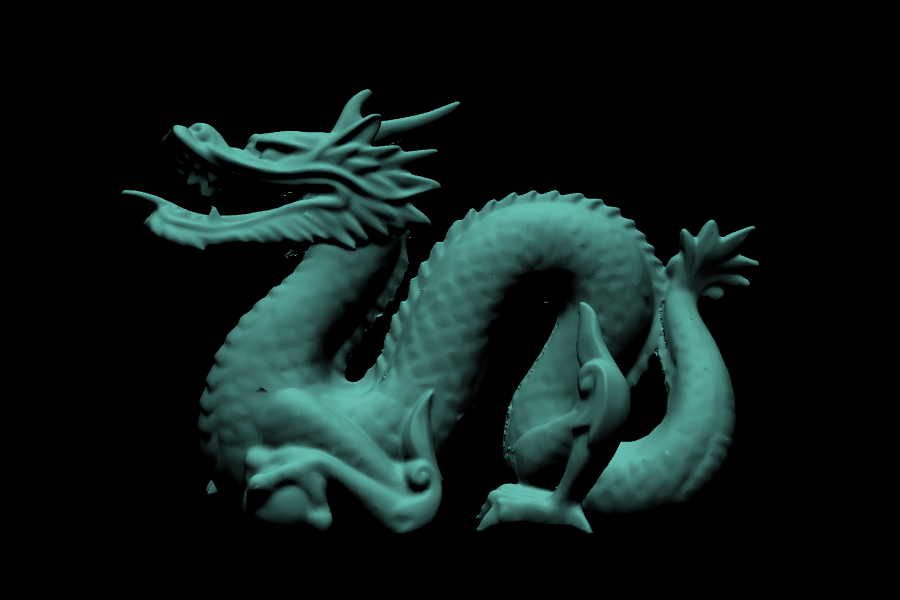
\includegraphics[width=\textwidth]{img/difuso}
   \caption{Reflexión difusa.}
   \label{fig:2c}
 \end{subfigure}
~
 \begin{subfigure}[b]{0.2\textwidth}
   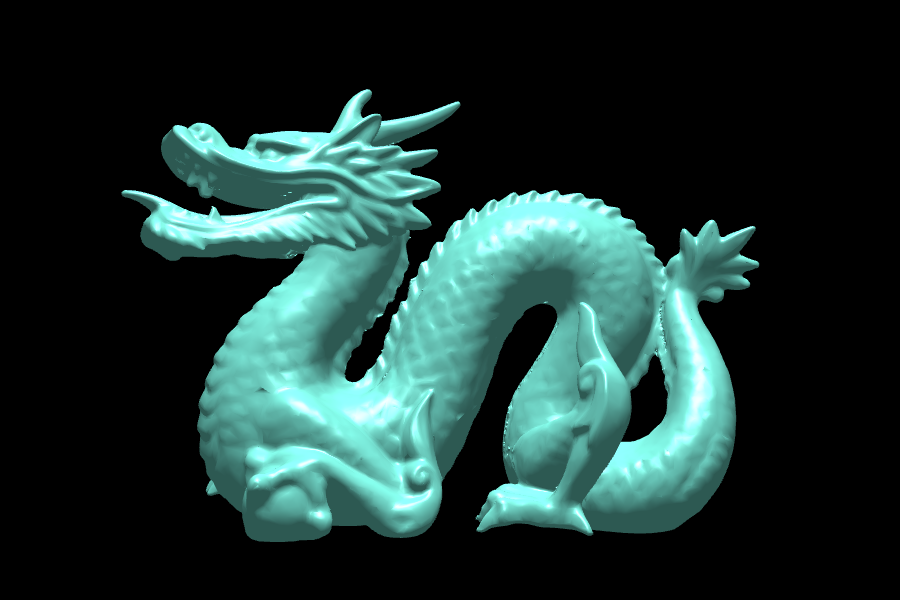
\includegraphics[width=\textwidth]{img/completo}
   \caption{Modelo completo.}
   \label{fig:2d}
 \end{subfigure}
    
  \caption{Componentes del módelo de iluminación de Phong.}
  \label{fig:two}
\end{figure}

También por regla general usamos entornos flotantes para poner Figuras, Tablas o pedazos de código.
Esto quiere decir que tenemos que usar especificadores como guías para que \LaTeX{} sepa dónde ponerlos exactamente en el texto.
Puedes consultar más de eso en \href{https://en.wikibooks.org/wiki/LaTeX/Floats,_Figures_and_Captions}{este} wikilibro.

\item Así es como se cita un libro: éste ejemplo fué tomado de~\cite{Devore2012}.
También hay un ejemplo de como hacer que un libro aparezca en las referencias sin que esté citado explícitamente en el texto.

Por último, este es un ejemplo de una tabla muy elegante: Cuadro~\ref{tab:exey}.
Hace uso del paquete \href{https://ctan.org/pkg/booktabs}{booktabs} por que las tablas predeterminadas en \LaTeX se ven muy anticuadas.
Debes de consultar este \href{https://jdhao.github.io/2019/08/27/latex_table_with_booktabs/}{post} y leer esta \href{https://people.inf.ethz.ch/markusp/teaching/guides/guide-tables.pdf}{presentacion} si vas a uasr muchas tablas en tu tesis.

\begin{table}[htb]
  \begin{center}
    \begin{tabular}{l | r r r r r}
      \toprule
      Source & \textbf{DF} & \textbf{SS} & \textbf{MS} & \textbf{F} & \textbf{P-value} \\
      \midrule
      \textbf{Model} & 2 & 0.00318564 & 0.00159282 & 7.72 & 0.0014 \\
      \textbf{Error} & 42 & 0.00866760 & 0.00020637 &  & \\
      \midrule
      \textbf{Total} & 44 & 0.01185324 &   &  & \\
      \bottomrule
    \end{tabular}
  \end{center}
\caption{Tabla Anova para un ejercicio imaginario}
\label{tab:exey}
\end{table}

\item En éste ejercicio, daré algunos tips enfocados a las ciencias de la computación.
Este ejemplo también demuestra como poner \say{comillas} en \LaTeX{}

Primero voy a mostrar cómo incluir algoritmos en forma de pseudocódigo.
Y desde luego se incluyen en el índice y se pueden referencias así: 
El Algoritmo~\ref{alg:euclid} es el primer algoritmo en la historia.
Se puede referenciar una línea del algoritmo.
El ciclo while termina en la línea line~\ref{euclidendwhile}.
Las ídeas las tomé de este enlace \href{https://en.wikibooks.org/wiki/LaTeX/Algorithms#Typesetting_using_the_algorithmicx_package}{wikibook} y de éste \href{https://tex.stackexchange.com/questions/229355/algorithm-algorithmic-algorithmicx-algorithm2e-algpseudocode-confused}{post}.

El entorno de algoritmo como flotante puede salirse de los márgenes de una pagina si no lo configuras correctamente.
Hay un \href{https://tex.stackexchange.com/questions/350434/adjust-width-of-algorithm-float}{truco} para hacerlo entrar en un cierto ancho.
Sin embargo, recomiendo usar el truco como última alternativa.
En estos ejemplos no fue necesario.

\begin{algorithm}[H]
\caption{Algoritmo de Euclides}
\label{alg:euclid}
\begin{algorithmic}[1] % El número le dice al entrono desde que numero empezar a contar. Si le pones 0 omite los números
    \Procedure{Euclid}{$a,b$} \Comment{El g.c.d. de $a$ y $b$}
    \State $r\gets a \bmod b$
    \While{$r\not=0$} \Comment{Si $r = 0$ ya tenemos la respuesta}
        \State $a \gets b$
        \State $b \gets r$
        \State $r \gets a \bmod b$
    \EndWhile\label{euclidendwhile}
    \State \textbf{return} $b$\Comment{$gcd = b$}
    \EndProcedure
\end{algorithmic}
\end{algorithm}

\item Aquí se muestra cómo incluir código fuente usando el paquete minted.
Este es un ejemplo en el lenguaje C.
\begin{listing}
\begin{minted}{cpp}
int main() {
  printf("hello, world");
  return 0;
}
\end{minted}
\caption{Un programa de ejemplo en C}\label{lst:hello}
\end{listing}

Este es otro ejemplo de cómo incluir Python dentro de un párrafo: \mintinline{python}{print(x**2)}.
Finalmente, lo más útil es incluir el código fuente desde un archivo externo: Vean  el Listado~\ref{lst:example} como ejemplo.
Me ayude muchisimo de \href{https://tex.stackexchange.com/questions/252263/alignment-of-minted-line-numbers}{aquí} y de la \href{https://www.overleaf.com/learn/latex/Code_Highlighting_with_minted}{ayuda de Overleaf}.
Observa la configuración que hice en el archivo \verb|tarea.sty| para ver cómo obtuve el resultado del Listado~\ref{lst:example}.

\begin{listing}
\inputminted[
  firstline=54, %If you omit this two fields, the whole file is pulled
  lastline=68
  ]{cpp}{src/GccTest.cpp}
  \caption{Una implementación defectuosa de insertion sort}\label{lst:example}
\end{listing}

\end{enumerate}

% Añade una entrada a las referencias, aun cuando no esta citado explícitamente
\nocite{Ross2012}
% Añade la bibliografía
\printbibliography
\end{document}
